\begin{savequote}[8cm]
Alles Gescheite ist schon gedacht worden.\\
Man muss nur versuchen, es noch einmal zu denken.

All intelligent thoughts have already been thought;\\
what is necessary is only to try to think them again.
  \qauthor{--- Johann Wolfgang von Goethe \cite{von_goethe_wilhelm_1829}}
\end{savequote}

\chapter{\label{ch:2-litreview}Background}

\minitoc
 This chapter summarises the main aspects of the tropical circulation and of the global monsoon. Then, the relevant background of the characteristics of American monsoon system and outstanding issues is given. 
\section{The tropical circulation and the global monsoon}\label{sq:bk_tropics}

Tropical climate is characterized by the strong incoming solar insolation year-round which makes the tropics the warmest region of the planet. 
The differential heating between the tropics and higher latitudes drives  a meridional transport of energy by the atmosphere. 
The tropical oceans that receive such a strong solar insolation exhibit strong evaporative fluxes. The in combination with the differential heating of land over ocean modulate the tropical circulation. % and ultimately convection. 
This tropical circulation can be described to a first order through the zonal and meridional circulations known as the Hadley and Walker cells. 
 
The Hadley cell is the meridional overturning circulation that arises from the differential heating between the tropics and the midlatitudes. The Hadley cell is characterized by ascending motions in the tropics and descending motions in the subtropics, and acts to transport heat poleward from the equator \citep{lorenz1967}.  
The boreal summer Hadley cell, for instance,  is primarily a result of ascent in the Indian Ocean and the west Pacific regions with a minor contribution from ascending motions in Central and North America \citep{hoskins2020}. 

The Walker circulation is the zonal overturning circulation found in the equatorial Pacific Ocean characterized by ascending motion over the West Pacific and descending motions over the East Pacific\citep{bjerknes1969,gill1980}. The dynamic and thermodynamic effects of the location and strength of convection in the Walker circulation have strong impacts across all the tropics and also the extratropics \citep{cai2019pantropical}.


\begin{figure}
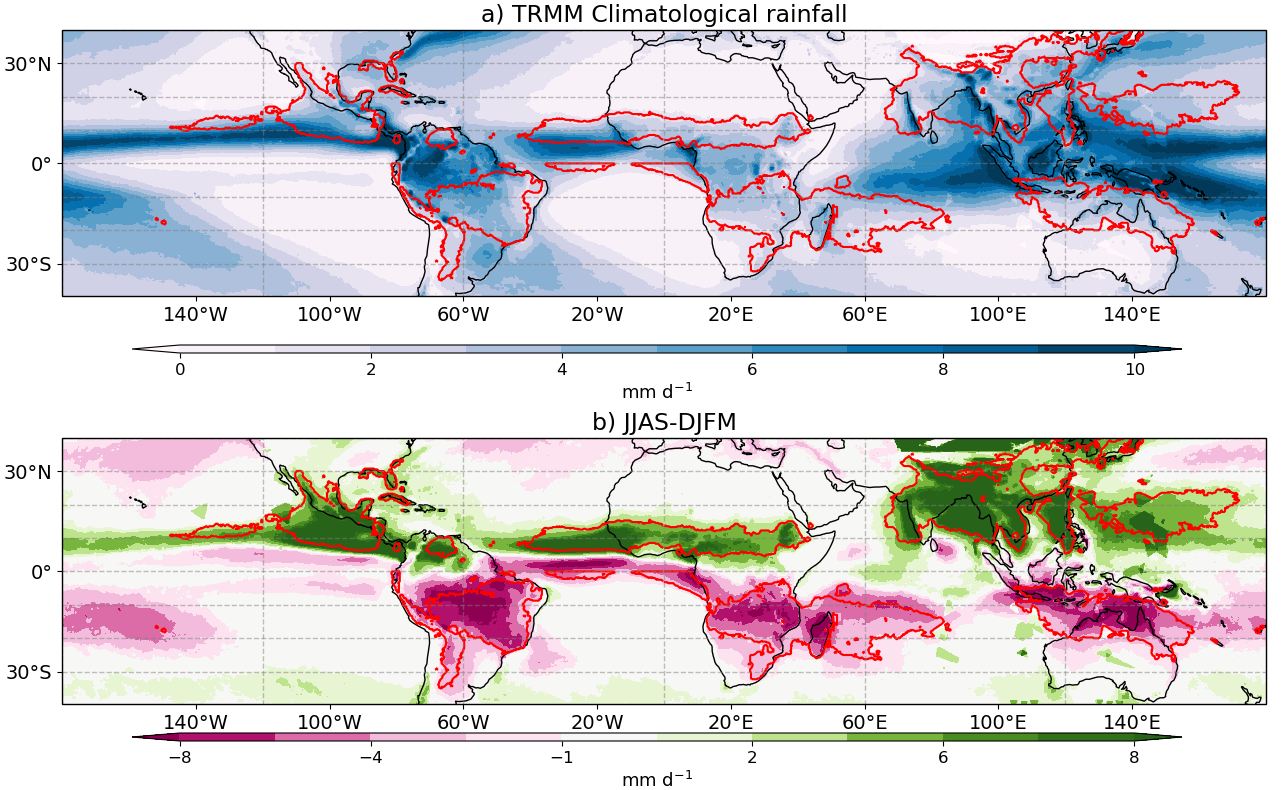
\includegraphics[width=\linewidth]{figures/trmmclima.png}
\caption{a) Climatological mean annual rainfall rates in the tropics in the TRMM dataset (1999-2018). b) The mean rainfall rate difference between boreal summer (JJAS) and austral summer (DJFM). The red contours highlight the regions where the summer rainfall amount accounts for more than 55\% of the total annual rainfall accumulation. }
\label{fig:monsoon}
\end{figure}

The Inter-tropical Convergence Zone (ITCZ) is a band of precipitation that migrates meridionally with the seasons \citep{schneider2014}. The ITCZ is arguably one of the most relevant features of tropical climate because tof the strong influence on the low- and upper-level circulation associated with ITCZ and the fact that the vast majority of rainfall in the tropics is due to convection in the ITCZ. The ITCZ is characterized by a strong convergent flow in the low levels and a strong divergent flow at upper levels. 
The meridional migration of the ITCZ, as well as the mean latitude of the ITCZ, results from the energy and momentum balances so that the ITCZ is predominantly north of the equator because of the inter-hemispheric temperature contrast \citep{donohoe2013,bischoff2016}.

The traditional view of a monsoon is that of a large-scale land-sea breeze associated with the different heatings of the land and the ocean that force a seasonal reversal of the winds. However, this framework has recently been challenged by the notion that monsoons are simply a manifestation of the ITCZ migration \citep{gadgil2018}. This has created the concept of the global monsoon as a phenomenon that exists all across the continental tropics \citep{zhou2016,gadgil2018}. 

The global monsoon refers to the those regions of the planet where more than 70\% of the total annual rainfall falls during the summer season \citep{zhou2016,wang2017}.
Figure \ref{fig:monsoon} shows the global monsoon as depicted by the TRMM dataset. By this definition, the majority of the regions over land between 5 and 10 degrees away from the equator are part of the global monsoon.

A regional monsoon, such as the Indian Monsoon, is then a subset of the global monsoon with unique regional characteristics that shape this monsoon different to other regional monsoons in terms of the seasonality, the strength and the dynamics. 

The American Monsoon System is then the regional monsoon that is located in the subtropics of North and South America. 
\section{The American Monsoon System}\label{sq:bk_ams}

The AMS is typically subdivided into the North and South American monsoon systems \citep{vera2006}.
The North American Monsoon is the main source of rainfall in south-western North America, extending north from central-west Mexico into the southwestern United States \citep{adams1997,stensrud1997,vera2006}.
 The seasonal cycle of rainfall in the North American Monsoon is characterised by a wet July-August-September season and significantly drier conditions during the rest of the year \citep{adams1997}.
A key aspect of this monsoon is the moisture advected by the low-level flow from the Gulf of California and the East Pacific Ocean and to a lesser extent the moisture mixed in the mid-troposphere from the Caribbean Sea and Gulf of Mexico \citep[e.g][]{stensrud1997,pascale2016,ordonez2019}.
%%

The South American Monsoon is a primary source of precipitation for South America, especially in the Amazon region \citep{gan2004,vera2006,jones2013}.
During austral summer (DJF), monsoon rainfall accounts for over 60\% of the total annual precipitation in the Amazon \citep{gan2004,marengo2012}, whereas
austral winter rainfall accounts for less than 5\% of the total annual rainfall \citep{vera2006}.
In the central Amazon, convective precipitation is observed from early October but the main rainy season extends from December to April \citep{machado2004,adams2013}, whereas convection in southeastern Brazil and Paraguay starts in November and peaks in January and February \citep{marengo2001,nieto2011}. 

\section{Review of the Midsummer drought}\label{sq:lit}


The seasonality of precipitation in northwestern Central America and southern Mexico fits the new definition of a monsoon characterized by the sharp contrast between the wet and dry seasons.
However, this region shows a unique climatological precipitation feature. After monsoon onset, rainfall decreases considerably around the midsummer; this decrease is followed by a secondary increase in precipitation in the late summer \citep{mosino1966}. 


These variations of precipitation are well known by local farmers who refer to the drier midsummer period as `El Veranillo' in Central America and `can\' icula' in southern Mexico because the drier period  coincides with the Canis Major constellation appearing in the sky \citep{dilley1996}. This feature of the seasonal cycle is most commonly referred to in the literature as Midsummer drought (MSD). 
Farmers in Central America who are subject to climatic stress due to droughts, have already perceived and adapted to changes in the characteristics of the rainy season, such as the timing and strength of the midsummer drought \citep{hellin2017,de2018,harvey2018}, but it is unclear whether these perceived changes are a real trend in the observations \citep{anderson2019multiscale}. 


Observations have characterised this feature in the climatological precipitation of several regions of Mexico, El Salvador, Belize, Guatemala, Cuba \citep[e.g.][]{mosino1966,magana1999,duranquesada2017,perdigon2018}.
However, notable differences in the seasonal cycle of precipitation have been found between the mainland and the Caribbean. The so-called first peak of precipitation occurs in May in Cuba and in June in northern Central America whereas the second peaks are observed in October and September for the mainland and the Caribbean, respectively. 

%The mechanisms that cause the MSD have been debated since the first observational descriptions of the phenomenon \citep[e.g.][]{mosino1966}, as studies that aimed to explain the physical mechanisms MSD have not yet reached a consensus.
 In spite of extensive research to understand the physical mechanisms associated with the MSD   \citep[e.g.][]{magana1999,giannini2000,gamble2008,ryu2014,herrera2015,maldonado2017,straffon2019}, debate remains over which is the leading-order mechanism that causes rainfall to decrease at midsummer and increase again at the end of the summer.  % why rainfall increases again at the end of the summer, the end of the MSD, and why this happens at this time of the year. 
Dynamical or the thermodynamical mechanisms have been put forth and different roles have been proposed for the Atlantic and the East Pacific Oceans \citep[e.g.][]{magana2005,gamble2008,herrera2015}. 

Fundamental questions remain unclear such  as whether the MSD is caused by two precipitation enhancing mechanisms \citep{karnauskas2013} or a mechanism that inhibits rainfall at midsummer \citep{duranquesada2017}. 
Furthermore, the association between the MSD in Central America and in the Caribbean is still disputed \citep{gamble2008}, as most studies suggest that the two regimes are unrelated and therefore two different explanations are required to account for the two MSDs in these regions. 

Any complete theory or conceptual model must account for the following characteristics of the seasonal cycle. First, the theory must explain the timing and strength of the first peak of rainfall. Second, the timing and strength of the MSD, i.e., what causes rainfall to decrease at midsummer. Finally, the theory must explain the timing and mechanism driving the second increase in precipitation after the midsummer. %The lack of a clear understanding of the processes that modulate the MSD makes climate change projections uncertain. 

\cite{magana1999} and \cite{magana2005} proposed a mechanism driven by radiative-convective feedbacks between the East Pacific SSTs and deep tropical convective clouds. The height and strength of convection, the incoming shortwave and the SSTs are strongly coupled in their framework. %Convection feedbacks with SSTs evaporation and
%moisture flux into the MSD region. 
The peak in  SSTs during May (Figure \ref{fig:csst}a) triggers evaporation and deep convection in the East Pacific ITCZ and Central America (Figure \ref{fig:msdcaribb}).
The high convective clouds produce a radiative cooling effect at the surface due to decreased incoming shortwave radiation (Figure \ref{fig:csst}d).
This cooling  decreases SSTs and deep convective activity and thus accounts for the modest decrease in rainfall during the midsummer.
The second peak in September is driven by the feedback effect caused by decreased frequency of tall convective clouds during July and August, as convective activity decreased during the MSD, which reduces the cooling effect of the clouds and increases incoming shortwave, SSTs and surface fluxes, eventually increasing precipitation \citep{magana1999}.



%have been linked to several sources of seasonal variability,
%but debate is far from uncontroversial as to which is the principal mechanism to account for the MSD.
 Other studies suggest the seasonal evolution of North Atlantic Subtropical High (NASH) and the associated geostrophic flow are the primary cause of the bi-modal regime, particularly for the MSD in the Caribbean  \citep[e.g.][]{mapes2005,gamble2008,curtis2008}.The NASH is a subtropical anticyclone in the Atlantic Ocean that shifts southwest early in boreal summer. The expansion and intensification of the NASH in boreal summer, according to this theory, strengthens the low-level trade winds, controlling the seasonal cycle of a low-level jet known as the Caribbean Low-Level Jet (CLLJ). 
 
 The CLLJ is key for regional variability and climate of the Caribbean, northern central America and southern United States, because the strength, height and direction determines the regional moisture transport \citep{giannini2000,martinez2019,garcia2020sub}. 
 The expansion of the western flank of the NASH is argued to strengthen the CLLJ which cools the SSTs, through the effect of wind stress and mixed-layer mixing \citep{gamble2008,martinez2019}.
The cooling of SSTs diminishes evaporation and therefore low-level moisture which leads to less precipitation, at least locally. Because the expansion of the NASH is closely aligned with the timing of the MSD in the Caribbean, the NASH effect on the CLLJ is argued to generate the bimodal regime of precipitation \citep{gamble2008,martinez2019}.

The moisture flow from the Caribbean Sea to the continent and the easternmost Pacific Ocean is another active topic of research \citep{hidalgo2015,corrales2020}. The effect of the SST gradient between the easternmost Pacific Ocean and the Caribbean Sea on the
  moisture flow across the continent is a relevant for variability on interannual time-scales \citep{martinez2020}. The Pacific Ocean is projected to warm more than the Caribbean Sea in future decades, which will change the SST gradient, strengthen the CLLJ and shifting the regional precipitation patterns \citep{corrales2020}.
  
 \cite{herrera2015} shows that during the drier months in Central America, stronger convective activity is found west of the Central American coast.  This evidence suggests that the coupling of EP SSTs to the gap flow that originated from the CLLJ in the Caribbean Sea controls the location of ascending and descending motions, thereby explaining some features of the Central American MSD. 
\cite{herrera2015} argued that the exit region of the CLLJ is located to the east of the region of strongest MSD signal, which suggests that the moisture divergence effect over the central American MSD is minimal. 



A different mechanism, proposed by \cite{karnauskas2013}, argues that the biannual crossing of the solar declination angle can control precipitation to the extent of explaining the bimodal characteristics of the seasonal cycle. In this mechanism, the MSD is driven by two precipitation enhancing periods that are separated by a relatively normal, and drier, period. This theory differs from those previously discussed which explained the MSD through mechanisms that inhibit convective activity in the midsummer whereas \cite{karnauskas2013} argues that the solar declination angle that crosses twice through Central America, once during June and a second time during September, increases convective activity during each crossing. 

The variations of incoming shortwave radiation associated with the declination angle modulate the SSTs, surface fluxes and therefore convective activity. In other words, the first crossing of the solar declination angle increases the incoming shortwave radiation which increases the SSTs, evaporation and precipitation, i.e., the first peak. The second crossing, similarly, explains the second peak as the second increase in incoming shortwave promotes more deep convection than during the MSD. 


Other mechanisms have been proposed arguing that the MSD is a result of the double crossing of the Intertropical Convergence Zone (ITCZ), the result of vertical wind shear affecting convective instability or the Saharan dust controlling  the microphysics of clouds \citep{angeles2010origins}.
For instance, \cite{perdigon2019} also finds a link between the frequency and spatial distribution of the first peak rainfall rates and the Madden-Julian Oscillation. 

\section{El Niño Southern Oscillation: impacts to the American monsoon system}
\label{sub:lit_enso}

 ENSO is the leading mode of interannual variability in the tropics which produces changes in the atmospheric circulation that impact most regions on the planet.
ENSO has motivated extensive research using GCMs to understand the mechanisms related the origin of ENSO \citep{christensen2017}, the feedbacks and processes that phase-lock the phenomena \citep{neelin1998}, as well as how will ENSO characteristics change in the future \citep{cai2015a,santoso2017}.

 ENSO is the oscillation from a mean state of the Walker circulation and the SST gradient. El Niño was initially the term to refer to the SST changes and the Southern Oscillation (SO) is associated with changes in the zonal gradient of MSLP. Combined, El Niño and the SO compose the ENSO phenomenon.
 
 The most prominent characteristic of ENSO is the effect that zonal gradients of MSLP and SST have on the location and strength of deep convection in the equatorial Pacific \citep{trenberth1997,neelin1998}. As ENSO shifts from the positive to the negative phase, deep convection shifts along the equatorial Pacific, generating precipitation anomalies on inter-annual timescales \citep{neelin1998,wang2004}. In other words, ENSO poses a strong control on the location and strength of the Walker circulation which then produces effects in remote regions of the world where the Walker circulation is important, \textit{e.g.}, in West Africa \citep{ropelewski1986,ropelewski1987} or South America \citep{sulca2018}.
 


The period of ENSO of 2-7 years \citep{neelin1998,wang2004} was poorly represented in CMIP3 and CMIP5 models \citep{guilyardi2009}, particularly by models that had much stronger power spectrums than the observed.



\section{Stratosphere-Troposphere Coupling in the Tropics}

\begin{figure}
\centering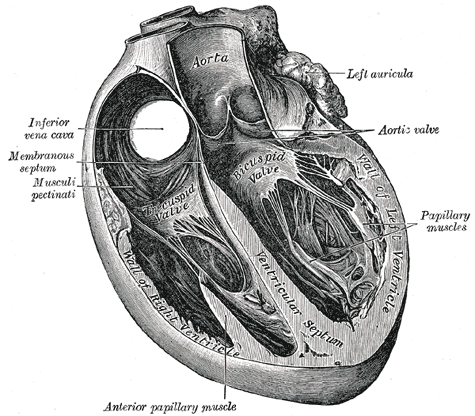
\includegraphics[width=0.7\textwidth]{figures/sample/Gray498.png} 
\caption[Four-chamber illustration of the human heart.]{Four-chamber illustration of the human heart.  Clockwise from upper-left: right atrium, left atrium, left ventricle, right ventricle.}
\label{fig:fourchamber}\end{figure}

The QBO is the dominant mode of tropical stratospheric variability which  modulates the characteristics of the tropopause in the tropics \citep{baldwin2001,tegtmeier2020} such as height and cold point temperature. 
Observations have shown an influence of the QBO on deep convective features such as monsoons \citep{giorgetta1999}, tropical cyclones \citep{chan1995} and the Walker circulation \citep{collimore2003}. More recently a link between the QBO and the Madden-Julian Oscillation (MJO) was discovered \citep{son2017} and motivated extensive research \citep[see e.g.][]{lee2018,wang2019,martin2020jgr}.

 The MJO in observations shows a stronger amplitude and more predictability during QBO E, but further inspection in cloud-permitting and forecast models have not provided conclusive answers to this puzzle \citep{martin2019,martin2020jgr}. Questions still arise as to whether this tropical link is real or due to chance, for instance \cite{wang2019} argued that the increased predictability of the MJO under the QBO E phase was included in the initial conditions, and thus not a result of a mechanistic effect of the QBO on the MJO. More generally, whether the QBO has a considerable effect on deep convection in general is debated as several plausible mechanisms exist in the literature \citep[see e.g.][]{nie2015} such as the effect of wind shear, the tropopause height, the cold-point temperature, static stability and/or feedbacks with very high cirrus and cumulunimbus clouds. 

The use of climate models to understand these tropical teleconnections of the QBO has proven difficult due to biases in both the MJO and the QBO representations. State-of-the-art CMIP6 models struggle to reproduce several of the characteristics of the QBO \citep{richter2020}. For instance,  weaker temperature QBO signals in the lowermost tropical stratosphere in the models, e.g., compare the QBOE-W difference plot in Figure \ref{fig:qbo}. The weaker temperature signal may be key for possible biases in the tropical QBO links discussed above, such as the the QBO-MJO link which is missing from CMIP6 models \citep{kim2020} and from seasonal prediction forecast models \citep{wang2019,martin2020jgr}. 